\chapter{Results}
\label{chapter:results}

%\emph{The chapter presents data preparation results for QGIS, PROWAT, and Pastas time series modeling. As well as outcomes of the QR factorization method for the study areas Rozenburg and Heijplaat.}

\section{Rozenburg}
\subsection{QGIS and PROWAT}
Figure \labelcref{beforeroz} represents a multi-colored scatter plot, showing the groundwater level [m NAP] over time [days]. Each colored dot represents an individual data point from a unique monitoring well, see legend on the right side of the figure. A wide array of groundwater levels is depicted, ranging from -1.0 to +3.0 m NAP. \\
\\
Plot \labelcref{beforeroz} visualizes the variation in groundwater levels between different monitoring wells. The legend explains a range of colors for the unique monitoring wells, that counts to 29 in the study area Rozenburg. The function of the groundwater level is indicated by the colored dot for every monitoring well. When no dot is present, it means that no data is available for this specific measurement date. Several monitoring wells perform constant groundwater levels, while other monitoring wells have abundant fluctuations in their function. Dense clustering of data points might suggest that measurements were taken frequently over time. The variety of colors allows for the possibility to compare groundwater level fluctuations between monitoring locations within the neighborhood. 

\begin{figure}[h]
    \centering
    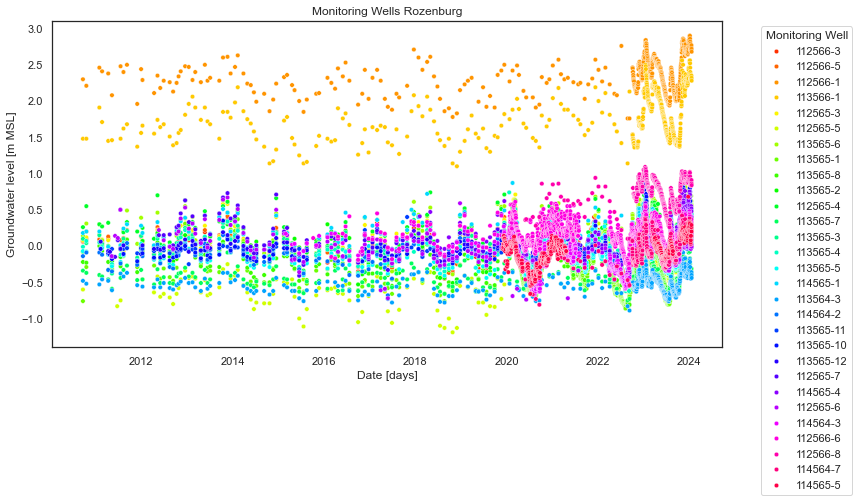
\includegraphics[width=0.80\linewidth]{frontmatter/Rozenburg-fig/rozscatter.png}
    \caption{Observed data for 29 monitoring wells in Rozenburg.}
    \label{beforeroz}
\end{figure}\\

\subsection{Pastas time series modeling}
The bar plot displays the recharge rates [m/day] over a period from 2010-2024. The x-axis represents the time period from 2010-2024 with the dates labeled on the x-axis. The y-axis quantifies the recharge rate with values ranging from 0 to a maximum of 0.07 m/day. The bars shows the variability in recharge rates over time, where some years experience peaks in recharge (higher recharge rates), which can be due to increased precipitation. As can be seen from \labelcref{recharge}, the data is dense, indicating frequent measurements by KNMI. The pattern of the bars reflects seasonal changes. Lower values are more frequently observed, possibly indicating a baseline level of recharge over the years. Two additional figures (\labelcref{P} and \labelcref{ET}) of precipitation and potential evaporation data are visualized as well. The data of these figures is combined to determine the recharge rate in the municipal area. 

\begin{figure}[htbp]
    \centering
    \includegraphics[width=0.80\linewidth]{frontmatter/Rozenburg-fig/Recharge.png}
    \caption{Recharge [m/day] over a period of 2010-2024, measured by KNMI weather station 344 in Rotterdam, The Netherlands.}
    \label{recharge}
\end{figure}

\begin{figure}[htbp]
    \centering
    % First figure
    \begin{minipage}{0.45\textwidth}
        \centering
        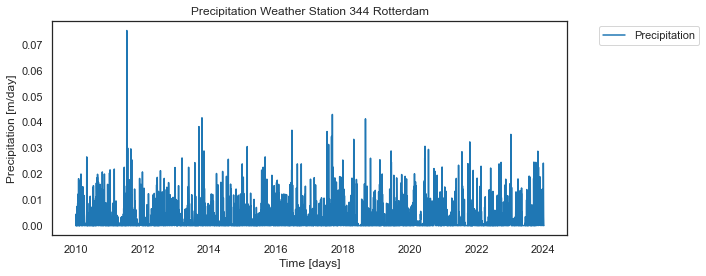
\includegraphics[width=\linewidth]{frontmatter/Heijplaat-fig/P.png}
        \caption{Precipitation [m/day] over a period of 2010-2024, measured by KNMI weather station 344 in Rotterdam, The Netherlands. }
        \label{P}
    \end{minipage}\hfill
    % Second figure
    \begin{minipage}{0.45\textwidth}
        \centering
        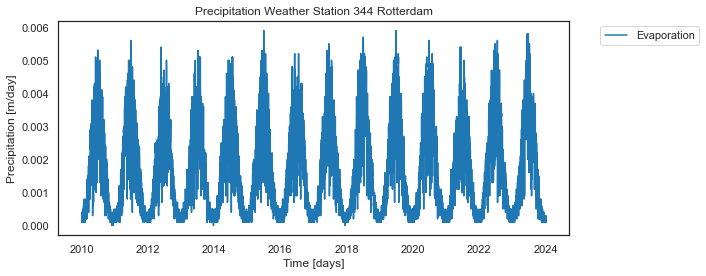
\includegraphics[width=\linewidth]{frontmatter/Heijplaat-fig/ET.png}
        \caption{Potential evaporation [m/day] over a period of 2010-2024, measured by KNMI weather station 344 in Rotterdam, The Netherlands.}
        \label{ET}
    \end{minipage}
\end{figure}

\subsubsection{Reversed forecasting}
Reversed forecasting, or also known as backcasting, of the observed GWL data is a feature in the Pastas Python package. The process is applied for every unique monitoring well within the case study area. For every well, three types of visualizations are generated: 1) Backcasting for data logger data; 2) Backcasting for the manually collected data; 3) A combination figure of figures 1 and 2 combined, see figures \labelcref{dl}-\labelcref{combi}. Monitoring well 112566-5 shows an example of the three visualized figures. The following applies for all three figures: The x-axis includes a period of 2010-2024 and the y-axis shows the simulated GWL data [m NAP].

\begin{figure}[htbp]
    \centering
    % First figure
    \begin{minipage}{0.32\textwidth}
        \centering
        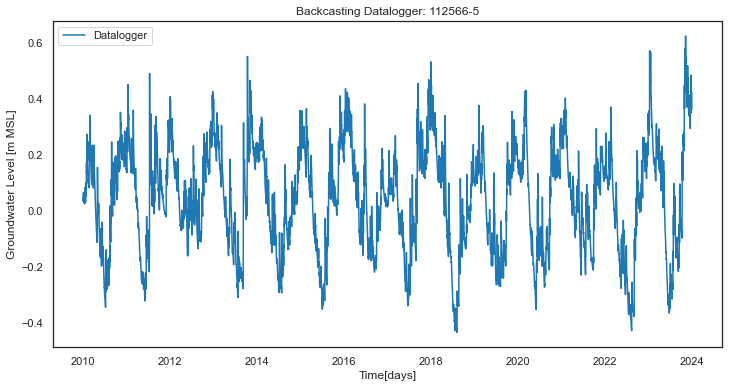
\includegraphics[width=\linewidth]{frontmatter/Rozenburg-fig/Figure 2024-03-12 093200 (180).png}
        \caption{Reversed forecasting data based on datalogger data for monitoring well 112566-5.}
        \label{dl}
    \end{minipage}
    \hfill
    % Second figure
    \begin{minipage}{0.32\textwidth}
        \centering
        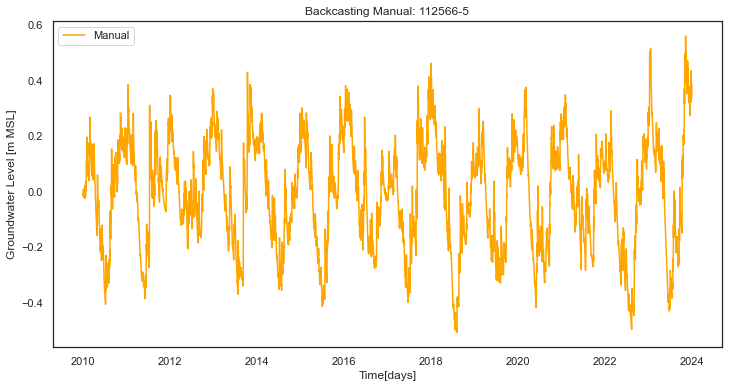
\includegraphics[width=\linewidth]{frontmatter/Rozenburg-fig/Figure 2024-03-12 093200 (209).png}
        \caption{Reversed forecasting data based on manual measurement data for monitoring well 112566-5.}
        \label{hp}
    \end{minipage}
    \hfill
    % Third figure
    \begin{minipage}{0.32\textwidth}
        \centering
        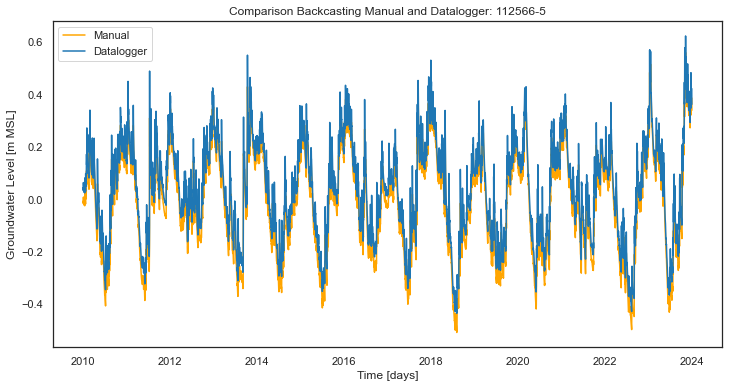
\includegraphics[width=\linewidth]{frontmatter/Rozenburg-fig/Figure 2024-03-12 093200 (238).png}
        \caption{Reversed forecasting data based on manual measurement data and datalogger data for monitoring well 112566-5.}
        \label{combi}
    \end{minipage}
\end{figure} \\
\newpage
\subsubsection{Performance metrics}
The bar plot \labelcref{bar1} and \labelcref{bar2} shows the two metrics RMSE and R$^2$ for all unique monitoring wells. In figure \labelcref{bar1}, a first overview is given of the t-Test with a distinction between RMSE and R$^2$ and an additional distinction between data loggers and manually collected wells. In figure\labelcref{bar1}, the R$^2$ value (orange bar) of all monitoring wells seems higher than the values of the RMSE (blue bar) of the same monitoring wells. Figure \labelcref{bar2} encompasses four categories: 1) manual-rmse; 2) manual-rsq; 3) datalogger-rmse; 4) datalogger-rsq. From this figure it is not clear if one of the datagroups has a better model performance, the performance of every model statistic differs between the monitoring wells. An additional bar plot, figure \labelcref{barevp} describes the EVP [\%] across the dataset. The EVP compares the variance of the observed data and the variance of the residual data across the 29 monitoring wells \cite{asmuth-2021}. It is not clear how the values relate to each other, because there is a distinction between the datalogger and manual collection method. A low EVP might indicate that data could be missing in the dataset, the spatial pattern could be a possible reason. A statistical t-Test is a follow-up to identify and statistically substantiate the difference in performance between the datagroups. Based on the results of the barplot, the decision was made to execute further statistical tests. A Welch's t-Test was carried out, leading to the following results. The Welch's t-Test uses an  \(alpha = 0.05\).
\begin{figure}[h]
    \centering
    \begin{minipage}{0.48\textwidth}
        \centering
        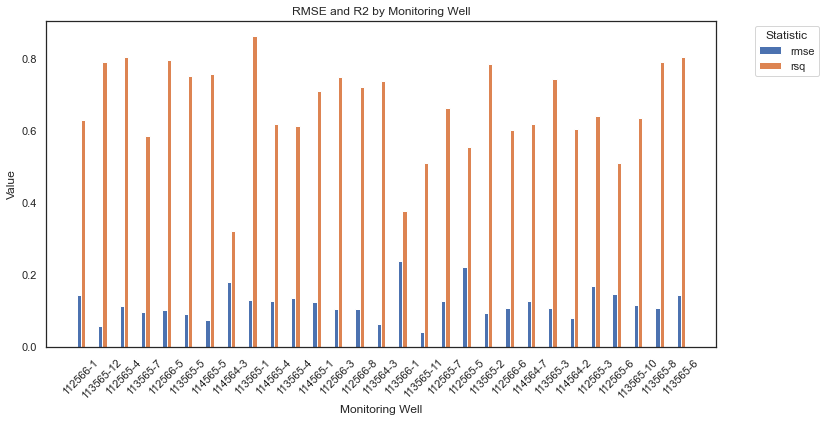
\includegraphics[width=\linewidth]{frontmatter/Rozenburg-fig/rmser2roz.png} % Adjust the file name or path as needed.
        \caption{Bar plot showing the metrics RMSE and $R^2$ for 29 monitoring wells.}
        \label{bar1}
    \end{minipage}\hfill
    \begin{minipage}{0.50\textwidth}
        \centering
        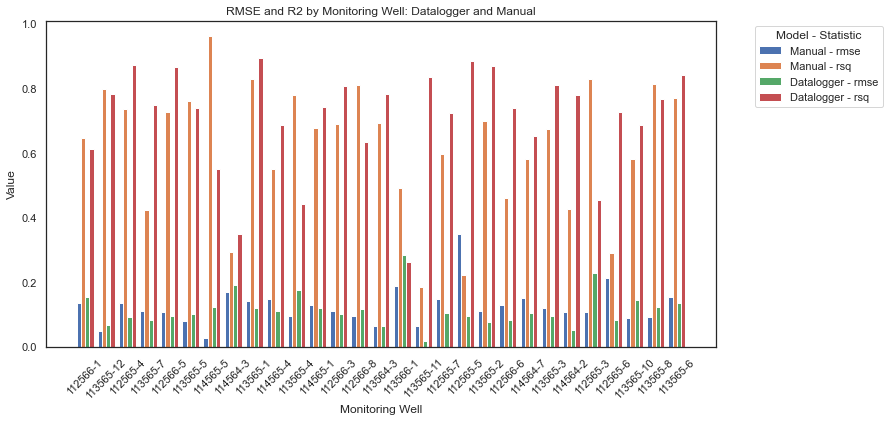
\includegraphics[width=\linewidth]{frontmatter/Rozenburg-fig/rmser2roz2.png} % Adjust the file name or path as needed.
        \caption{Bar plot showing metrics RMSE and $R^2$ for 29 monitoring wells with a division in data logger and manual collection method.}
        \label{bar2}
    \end{minipage}
\end{figure}

\begin{figure}[h]
    \centering
    \begin{minipage}{0.48\textwidth}
        \centering
        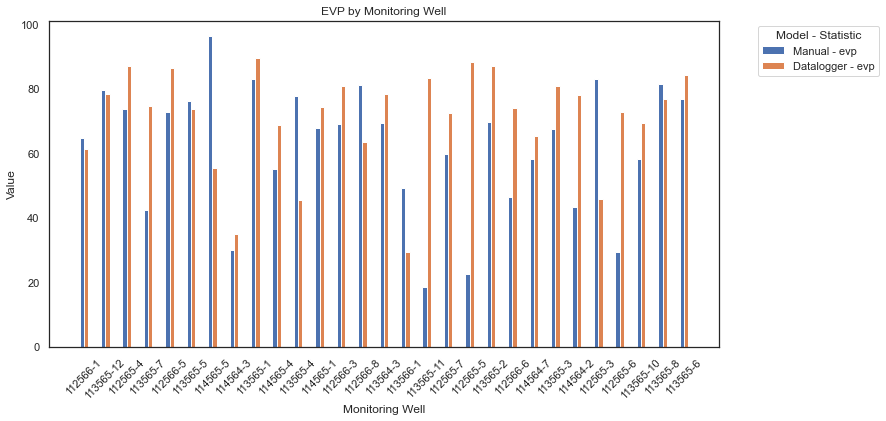
\includegraphics[width=\linewidth]{frontmatter/Rozenburg-fig/evproz2.png} % Adjust the file name or path as needed.
        \caption{Bar plot showing metric EVP for 29 monitoring wells.}
        \label{barevp}
    \end{minipage}\hfill
\end{figure}
\clearpage
\noindent
Figure \labelcref{welch} displays the result of the Welch's t-Test, based on \(alpha = 0.05.\) The results of the performance metrics are labeled as RMSE, R$^2$, and EVP. Each performance metric provides the results of the t-statistic and p-value of the Welch's statistical test. The RMSE (blue section), explains that the t-statistic is negative. This result could indicate that the data loggers have a lower mean RMSE than the manual collection method. The p-value is higher than \(alpha = 0.05\). A p-value higher than the set alpha explains that no significant difference is present between the data loggers and manual collection method. The R$^2$ (orange section) explains that the t-statistic is positive, indicating a higher mean R$^2$ for the data loggers than the manual collection method. The p-value is slightly higher than \(alpha = 0.05\), indicating no significant difference. The last metric is the EVP (green section). The t-statistic of the EVP has a positive value, suggesting that the data loggers might have a higher mean EVP than the manual collection method. The p-value of 0.065 is very close to 0.05, but resulting in no significant difference. 
\begin{figure}[htbp]
    \centering
    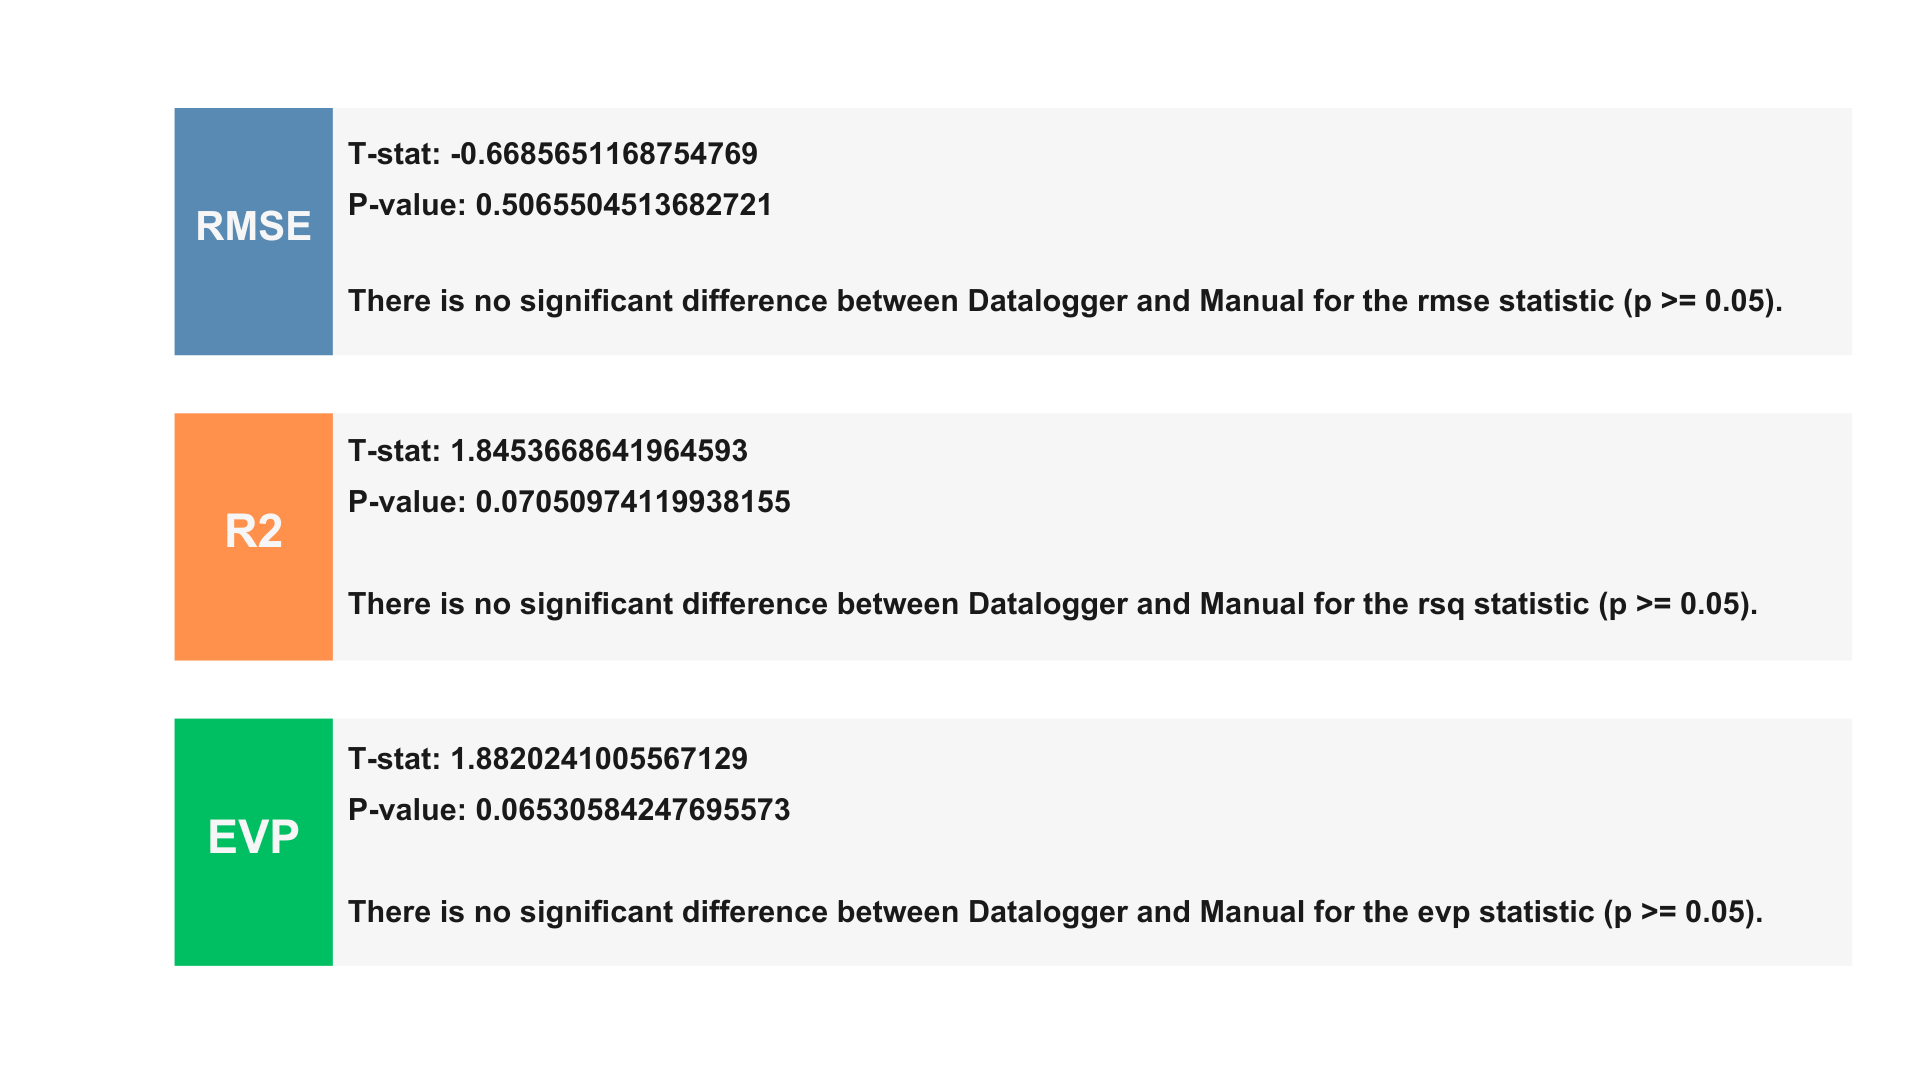
\includegraphics[width=0.80\linewidth]{frontmatter/Rozenburg-fig/sigroz.png}
    \caption{Overview of the performance of RMSE, $R^2$ , and EVP after the Welch's t-test and the difference between data loggers and manual collection method. }
    \label{welch}
\end{figure}\\
\\
\noindent
The Welch's t-Test does not reveal no substantial discrepancies between the data groups. None of the p-values are below the threshold value of 0.05. Despite statistical significance, factors as data availability and reliability are decisive. Hence, the data logger group is chosen, merging observed and simulated data into one dataset and excluding the manual measurement from the research. 

\subsubsection{Creation of a new data frame}
Scatter plot \labelcref{scatter} below, visualizes the observed data logger data with the blue scatter and the simulated data of the data logger is visualized by the orange scatter. On the x-axis the time period [days] is shown and on the y-axis the groundwater level [m NAP]. Figure \labelcref{scatter} visualizes only monitoring well 112566-5, the remaining monitoring wells of the neighborhood Rozenburg are available through \href{https://github.com/hannahwillemijn9/GWMNO-Rotterdam.git}{Github}.

\begin{figure}[htbp]
    \centering
    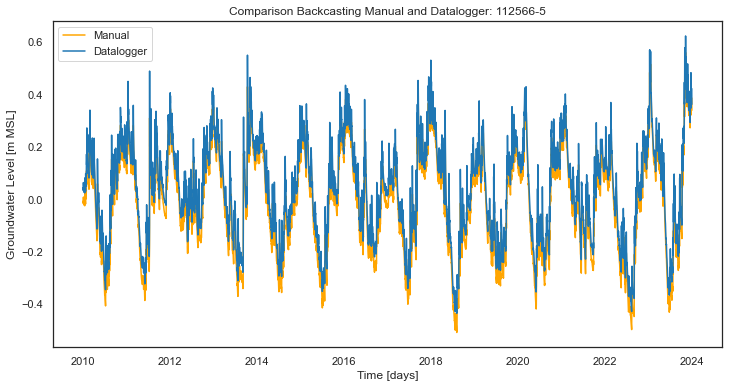
\includegraphics[width=0.80\linewidth]{frontmatter/Rozenburg-fig/Figure 2024-03-12 093200 (238).png}
    \caption{Scatter plot of simulated and observed data by data loggers for monitoring well 112566-5. The x-axis shows a period of 2020-2024 and the y-axis shows a range of -0.5 to 0.6 meters NAP. }
    \label{scatter}
\end{figure}
\newpage
\subsection{QR factorization}
Using QR factorization as a foundation, a hierarchical list of the monitoring wells in Rozenburg can be created. The optimal reduction percentage is determined and reduction tests can be executed, resulting in an overview of eliminated monitoring wells and their capability to reconstruct future groundwater levels in the network.

\subsubsection{1D hydrograph data}
Figure \labelcref{gwlroz} is a geographical representation visualizing the spatial distribution of monitoring wells in the neighborhood Rozenburg. Within the map, a scatter plot with a color scale represents the groundwater level measurements taken at the monitoring wells. The groundwater level has a range between -1.00 m to +3.00 m NAP. Each monitoring well represents a location as well as the color of monitoring well represents the value on the color scale. At the north side of the neighborhood, deviating groundwater level measurements can occur because of the elevation difference of the ground level, a digital terrain model of Rozenburg is displayed in figure \labelcref{AHNroz}.
\begin{figure}[htbp]
    \centering
    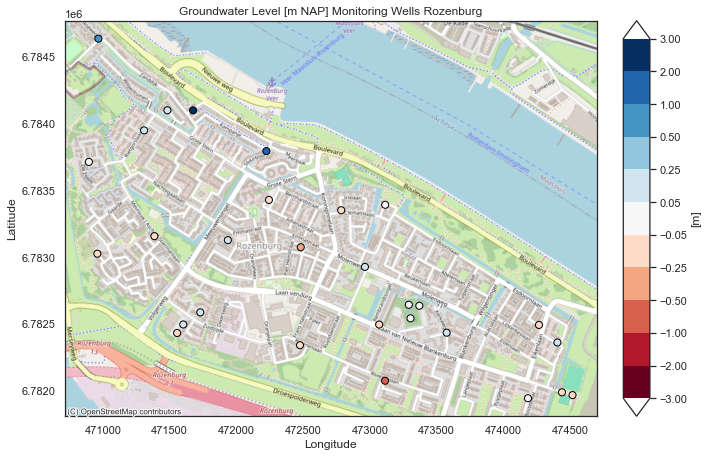
\includegraphics[width=0.75\linewidth]{frontmatter/Rozenburg-fig/gwlroz.png}
    \caption{Groundwater level [m NAP] across Rozenburg, using a color-coded system to represent the mean GWL observations for the 29 monitoring wells. Based on EPSG:28992/Amersfoort RD New.}
    \label{gwlroz}
    
\end{figure}

\subsubsection{Sampling data}
Preprocessing of the data includes transforming the data frame into an array, implementing both global and local centering methods, and splitting the dataset into an 80/20 ratio training and test set distribution. The result of the preprocessing is as follows, see table \labelcref{data}
\begin{table}[htbp]
\centering
\caption{Summary of sampling data.}
\label{data}
\begin{tabular}{|l|l|}
\hline
\textbf{Parameter}                           & \textbf{Value}                                \\ \hline
Sampling period                              & 2020-01-02 00:00:00 to 2024-01-01 00:00:00\\ \hline
Number of samples                            & 1462\\ \hline
Number of features (sensors)                 & 29                                            \\ \hline
Shape of X (samples, sensors)                & (1462, 29)\\ \hline
Min. and max. value                          & -0.8794576895779862 [m] ; 2.9179266529665524 [m]\\ \hline
Train data, Test data                        & 1169 , 293\\ \hline
Train data, Test data (percentage)           & 80\%, 20\%                                  \\ \hline
\end{tabular}
\end{table} 

\subsubsection{Hierarchy of monitoring wells}
A geographical representation of data points plotted on a x,y coordinate system is visualized in figure \labelcref{rankroz}. The horizontal axis is labeled as longitude and the vertical axis is labeled as latitude. The data points are scattered across the study area within the neighborhood Rozenburg. Each monitoring well is color-coded according to the color bar on the right side of the plot. The color indicates the rank of each monitoring well and has a range between dark blue for the lowest values (1) to yellow for the highest values (29). The distribution of the color code does not follow a clear pattern within the neighborhood boundary. Some clusters of higher or lower ranked monitoring wells are present. The monitoring wells with additional value are marked blue, while the monitoring wells that likely do not have additional value to the network are marked yellow. The most redundant monitoring wells appear to be located towards the southern edge of the neighborhood. At the southern side, and a single well in the north as well, monitoring wells are clustered and address a region of low data variability and flashiness.
\begin{figure}[h]
    \centering
    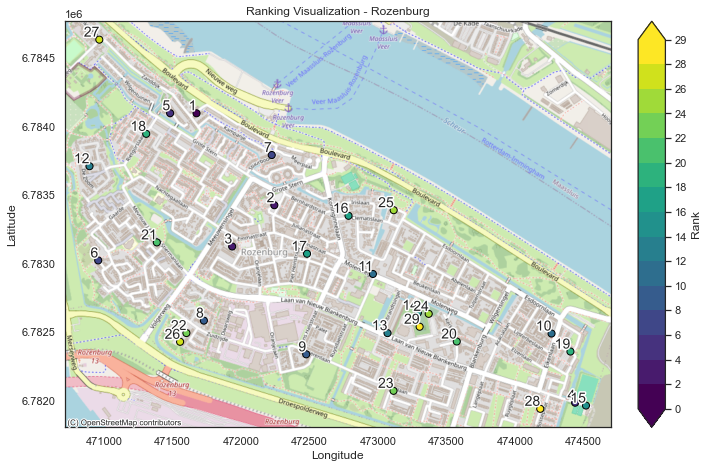
\includegraphics[width=0.8\linewidth]{frontmatter/Rozenburg-fig/rank.png}
    \caption{Visualization of the hierarchical list of 29 monitoring wells across Rozenburg. Based on EPSG:28992/Amersfoort RD New.}
    \label{rankroz}
\end{figure} 

\newpage

\subsubsection{Determining the optimal reduction rate}
In figures \labelcref{roz10} - \labelcref{roz90} , the reconstruction error of Rozenburg is displayed, plotting the number of monitoring wells on the x-axis against the root mean square error (RMSE) in meters on the y-axis. The line graph shows a decreasing function as the number of monitoring wells increases and the RMSE decreases, suggesting that more monitoring wells contribute to a lower reconstruction error in the data. In the figures, the orange marked point marks the optimal number of monitoring wells where the reconstruction error reaches the threshold that is indicated by the orange line. The threshold is an acceptable level of RMSE for the reconstruction process. The original groundwater monitoring network of Rozenburg includes 29 monitoring wells.
\newline
Starting with figure \labelcref{roz10}, a reduction of 10\% describes that 26 monitoring wells remain in the network and only 3 monitoring wells might be eliminated. The reconstruction error reaches a value below 0.02 meters. The RMSE in figure \labelcref{roz25} with a reduction of 25\%, explains that a number of 21 monitoring wells is the most optimal number with a removal of 8 monitoring wells.  Figure \labelcref{roz50} demonstrates a function based on a reduction percentage of 50\%. The RMSE decreases as more monitoring wells are added to the network. At the point of n=14 on the x-axis, an orange dot is indicated. Beyond this point, the decrease in RMSE slows down, suggesting returns on error reduction after a specific number of monitoring wells is reached. 

\begin{figure}[htbp]
    \centering
    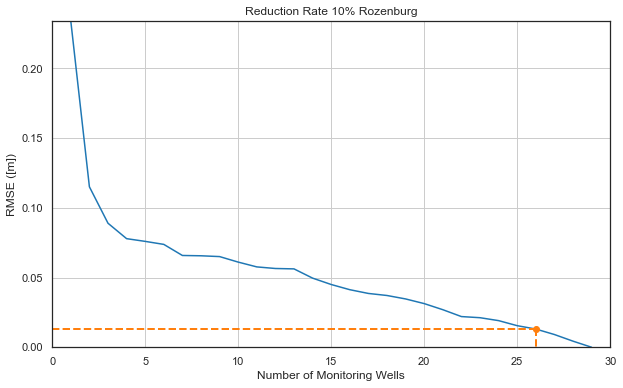
\includegraphics[width=0.48\linewidth]{frontmatter/Rozenburg-fig/new10.png}
    \caption{RMSE based on a network reduction of 10\%. The optimal number of wells is 26.}
    \label{roz10}
\end{figure}

    % Second Figure
    \begin{figure}[htbp]
    \begin{minipage}{0.48\textwidth}
        \centering % Centers the content of this minipage
        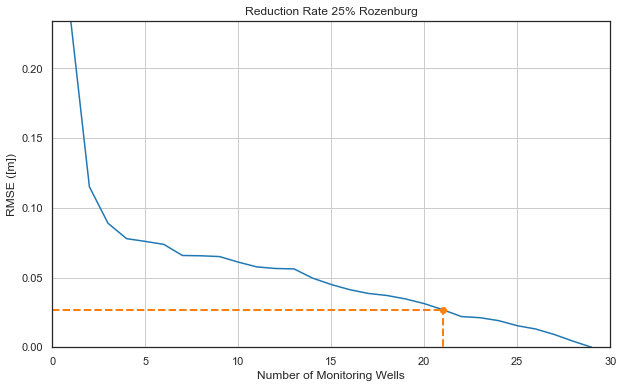
\includegraphics[width=\linewidth]{frontmatter/Rozenburg-fig/new25.png}
        \caption{RMSE based on a network reduction of 25\%. The optimal number of wells is 21.}
        \label{roz25}
    \end{minipage}
    % Third Figure
    \begin{minipage}{0.48\textwidth}
        \centering % Centers the content of this minipage
        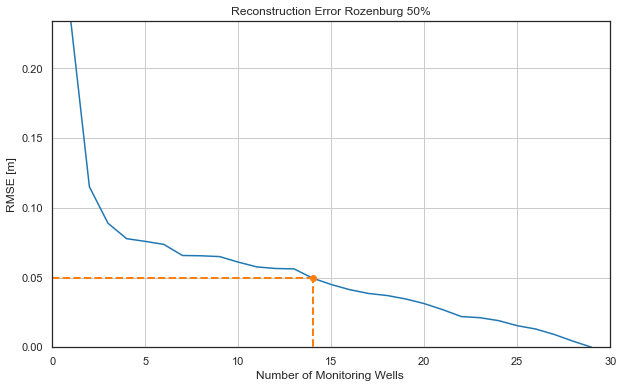
\includegraphics[width=\linewidth]{frontmatter/Rozenburg-fig/new50.png}
        \caption{RMSE based on a network reduction of 50\%. The optimal number of wells is 14.}
        \label{roz50}
    \end{minipage}
\end{figure}
\noindent
Figure \labelcref{roz75} displays a function where the RMSE decreases as the number of monitoring wells increases. The RMSE sharply declines as the monitoring well count approach reaches the point above 10 monitoring wells. This point is marked by the orange dashed line. The line marks the optimal number of monitoring wells where the reconstruction error reaches the threshold value. The threshold value is determined by the trade off between the maximum information value and minimum cost, in which the maximum information value is characterized by the reconstruction error and the minimum cost is equivalent to the number of monitoring wells. Initially, Rozenburg includes 29 monitoring wells. The results of the RMSE explain that only 7 monitoring wells will remain, 22 monitoring wells have to be removed from the local network if a reduction of 75\% is used in the approach. A reduction percentage of 75\% explains an equilibrium state between the number of monitoring wells and the reconstruction error that is achieved.
\newline
\newline
Continuing with figure \labelcref{roz90}, the reconstruction error for a reduction of 90\% is displayed. The figure plots the number of monitoring wells on the x-axis against the RMSE in meters on the y-axis. The line graph shows a sharp decreasing function in the RMSE as the number of monitoring wells increase. The orange marked dot marks the optimal number of monitoring wells where the reconstruction error reaches the threshold value that is indicated by the orange line. The threshold value is an acceptable level of RMSE for the reconstruction process. Initially, Rozenburg has 29 monitoring wells. The results of the RMSE calculation explains that a number of 2 monitoring wells will remain with this reduction rate, 27 monitoring wells will be removed from the local network with a reduction rate of 90\%.
\begin{figure}[htbp]
    \centering
    \begin{minipage}{0.48\textwidth}
        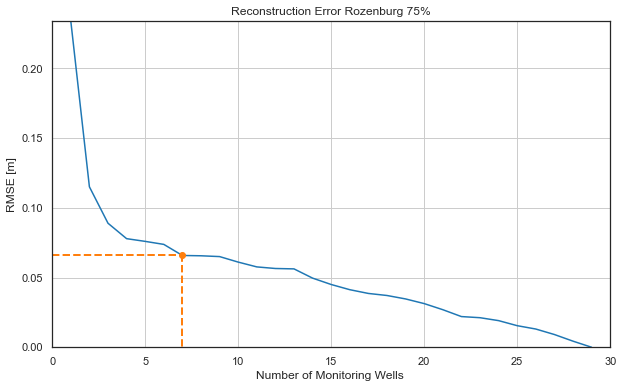
\includegraphics[width=\linewidth]{frontmatter/Rozenburg-fig/new75.png}
        \caption{RMSE based on a network reduction of 75\%. The optimal number of wells is 7.}
        \label{roz75}
    \end{minipage}\hfill
    \begin{minipage}{0.48\textwidth}
        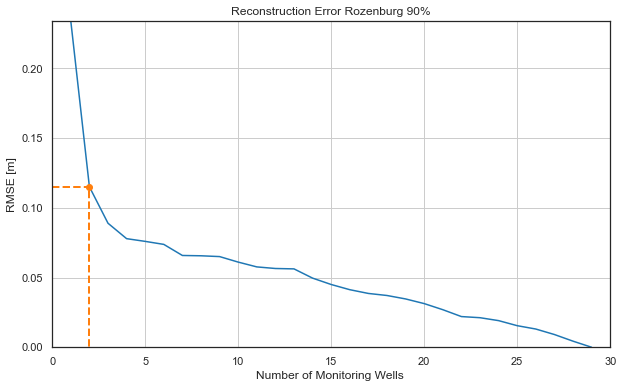
\includegraphics[width=\linewidth]{frontmatter/Rozenburg-fig/new90.png}
        \caption{RMSE based on a network reduction of 90\%. The optimal number of wells is 2.}
        \label{roz90}
    \end{minipage}
\end{figure}
\subsubsection{The optimal reduction rate}
The optimal reduction rate for a monitoring network consisting of 29 monitoring wells counts up to a value where the RMSE reach stabilization. Figure \labelcref{rmse} visualizes all reduction percentages between a range of 10-90\% with their corresponding reconstruction error and mean absolute error. \\
\\
A reduction percentage of 25\% implies that the optimal number of monitoring wells is 21, meaning that 8 monitoring wells might be eliminated, see figure \labelcref{roz25}. Additionally, the RMSE counts up to 0.027 meters. 
\begin{figure}[htbp]
    \centering
    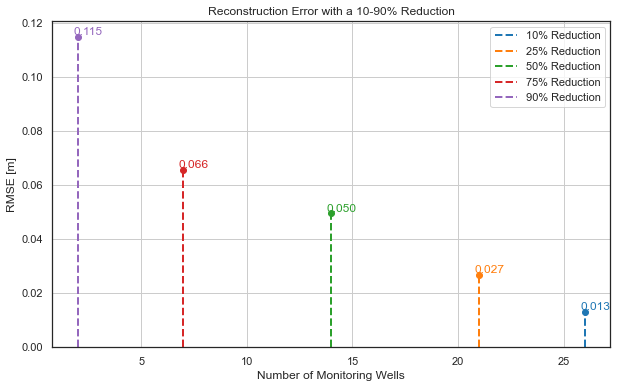
\includegraphics[width=0.5\linewidth]{frontmatter/Rozenburg-fig/rmseroz.png}
    \caption{Overview of the RMSE for a range of reductions (10-25-50-75-90\%). }
    \label{rmse}
\end{figure}
As stated in the chapter \textit{Research Methodology}, the reconstruction capability of the eliminated monitoring wells is tested through the creation of hydrographs. In figures \labelcref{roz1}-\labelcref{roz8}, hydrographs are shown. The hydrographs include a measured (blue line) and reconstructed (orange line) function. The reconstructed functions are based on observed data and the Goodness-of-Fit of the model. Performance metrics regarding the MAE, RMSE, $R^2$, and rBIAS determine the Goodness-of-Fit of the functions, they are available underneath the figures \labelcref{roz1}-\labelcref{roz8}. 
\newpage
\noindent
As can be seen from the figures, the plots have a comparable function; a decreasing groundwater level from April 2023 on and reaching the lowest groundwater level in July 2023. In August of the same year, the groundwater level increases again to high levels. At the end of August 2023, the groundwater level decreases again, but experiences peak values in October 2023. At the end of 2023, the groundwater levels are increasing again, but at this time of the year, the levels seem more constant. Based on the performance metrics of the potentially eliminated monitoring wells, it can be seen that the MAE and RMSE are constant values throughout the network. The MAE reaches a value of 0.04 meters and the RMSE counts up to 0.05 meters. The coefficient of determination differs for every monitoring well, but ranges between 0.79 and 0.95. An average of 0.905 [-] is calculated.
\begin{figure}[h]
    \centering
    % Row 1
    \begin{minipage}{0.48\textwidth}
        \centering
        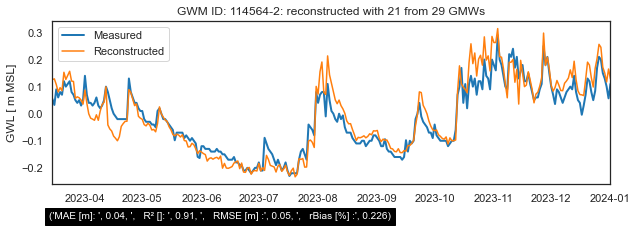
\includegraphics[width=\linewidth]{frontmatter/Rozenburg-fig/1145642roz.png}
        \caption{Eliminated monitoring well: 114564-2.}
        \label{roz1}
    \end{minipage}\hfill
    \begin{minipage}{0.48\textwidth}
        \centering
        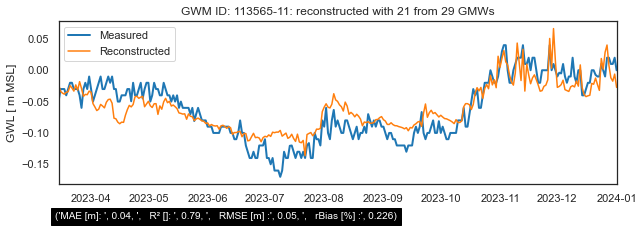
\includegraphics[width=\linewidth]{frontmatter/Rozenburg-fig/11356511roz.png}
        \caption{Eliminated monitoring well: 113565-11. }
        \label{113565-11}
    \end{minipage}
    
    % Row 2
    \begin{minipage}{0.48\textwidth}
        \centering
        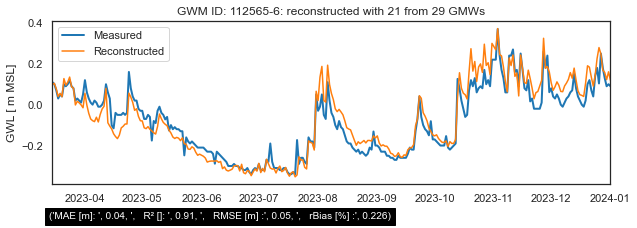
\includegraphics[width=\linewidth]{frontmatter/Rozenburg-fig/1125656roz.png}
        \caption{Eliminated monitoring well: 112565-6.}
        \label{112565-6}
    \end{minipage}\hfill
    \begin{minipage}{0.48\textwidth}
        \centering
        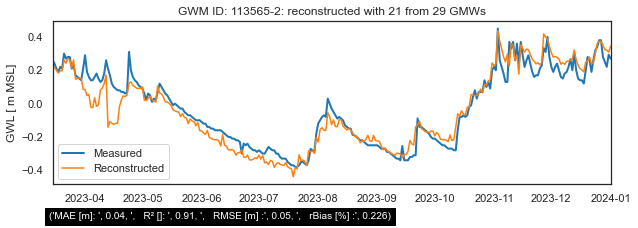
\includegraphics[width=\linewidth]{frontmatter/Rozenburg-fig/1135652roz.png}
        \caption{Eliminated monitoring well: 113565-2.}
        \label{113565-2}
    \end{minipage}
    % Row 3
    \begin{minipage}{0.48\textwidth}
        \centering
        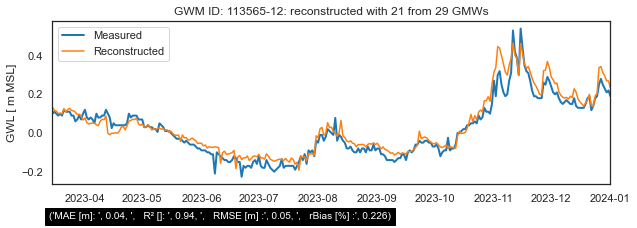
\includegraphics[width=\linewidth]{frontmatter/Rozenburg-fig/11356512roz.png}
        \caption{Eliminated monitoring well: 113565-12.}
        \label{113565-12}
    \end{minipage}\hfill
    \begin{minipage}{0.48\textwidth}
        \centering
        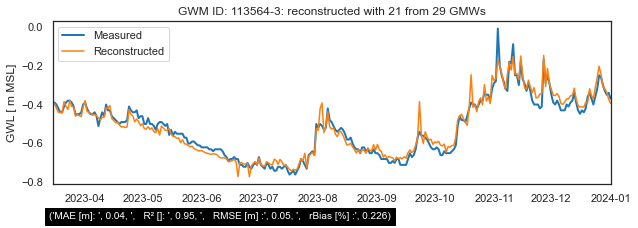
\includegraphics[width=\linewidth]{frontmatter/Rozenburg-fig/1135643roz.png}
        \caption{Eliminated monitoring well: 113564-3.}
        \label{113564-3}
    \end{minipage}

    % Row 4
    \begin{minipage}{0.48\textwidth}
        \centering
        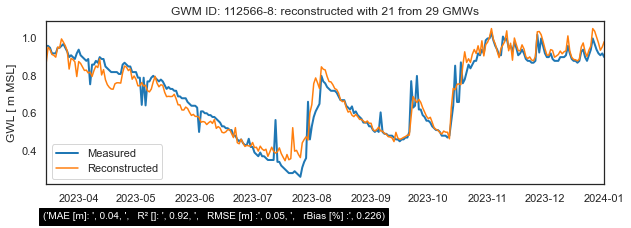
\includegraphics[width=\linewidth]{frontmatter/Rozenburg-fig/1125668roz.png}
        \caption{Eliminated monitoring well: 112566-8.}
        \label{112566-8}
    \end{minipage}\hfill
    \begin{minipage}{0.48\textwidth}
        \centering
        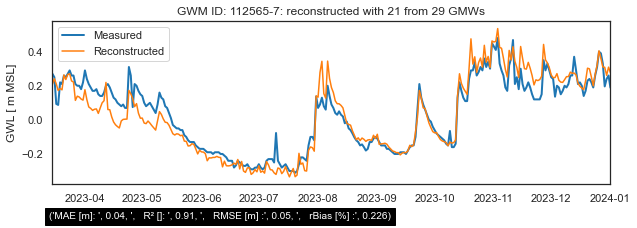
\includegraphics[width=\linewidth]{frontmatter/Rozenburg-fig/1125657roz.png}
        \caption{Eliminated monitoring well: 112565-7.}
        \label{roz8}
    \end{minipage}
\end{figure}\\
\\
The measured and reconstructed groundwater levels are tested with the Welch's t-Test to determine whether there is a case of a significant difference between the measured and reconstructed groundwater levels. The results are displayed in table \labelcref{welchroz}. Only 5 out of 8 eliminated monitoring wells experiences a significant difference between the measured and reconstructed groundwater level data. This means that the p-values of the monitoring wells are lower than \(alpha = 0.05\). 
\begin{table}[htbp]
    \centering
      \caption{Overview of statistical results of the eliminated monitoring wells with a network reduction of 25\%. The overview explains the p-value of the monitoring wells and if they experience a significant difference between the observed and reconstructed data.}
    \begin{tabular}{|c|c|} \hline  
         Monitoring Well& Result t-Test\\ \hline  
         112565-6& Significant difference (p-value = 0.002)\\ \hline  
         112565-7& No significant difference 
(p-value = 0.208)\\ \hline  
         112566-8& No significant difference 
(p-value = 0.115)\\ \hline  
         113564-3& No significant difference 
(p-value = 0.100)\\ \hline  
 113565-11&Significant difference (p-value = 0.036)\\ \hline 
         113565-12& Significant difference (p-value = 0.000)\\ \hline  
         113565-2& Significant difference (p-value = 0.002)\\ \hline  
         114564-2& Significant difference (p-value = 0.001)\\ \hline
    \end{tabular}

    \label{welchroz}
\end{table}
\newpage
\noindent
Figure \labelcref{rozbox} visualizes a box plot that displays the distribution of the performance metric $R^2$, the coefficient of determination, across the dataset after reduction of 25\% took place. On the y-axis, the score in meters is shown, which ranges between 0.785 and 0.952. The orange line explains a median value of 0.912. The whiskers at the bottom and top of the box do not have equal length. The whisker at the bottom reaches a value up to 0.785 to a score of 0.910. The box itself ranges between 0.912 and 0.929 [-].

\begin{figure}[htbp]
    \centering
    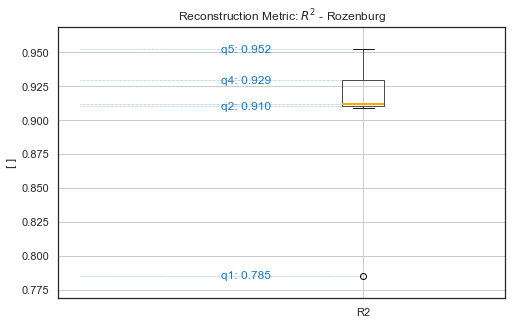
\includegraphics[width=0.5\linewidth]{frontmatter/Rozenburg-fig/boxroz.png}
    \caption{Performance metric $R^2$ for Rozenburg. 
    The orange line indicates the median value. The y-axis ranges from 0.785 to 0.952 [-].}
    \label{rozbox}
\end{figure}

\subsubsection{Mean Absolute Error of Reduction}
Based on a reduction percentage of 25\%, reconstruction hydrographs could be plotted in figures \labelcref{roz1}-\labelcref{roz8}. The extent to which the reconstructed groundwater level data corresponds to the actual observed data can be determined by the mean absolute error [meters]. The mean absolute error is calculated for every eliminated monitoring well. A color rank is visualized in figure \labelcref{maeroz} with the level of the calculated mean absolute error. Blue indicates a low MAE, while yellow indicates a high MAE. The visualization enables the identification of monitoring wells with higher or lower predictive accuracy, which could influence decision-making regarding the placement of future monitoring wells or the scope of maintenance efforts on existing wells. The MAE measures indirectly the performance of the monitoring well regarding data reconstruction. A high MAE in a network of lower MAE values can suggest a vulnerable monitoring well for external environmental factors. Monitoring wells with a high MAE can not be reproduced easily, because the prediction can be unreliable. The monitoring well that is marked with a yellow color indicates a higher MAE value compared to the other monitoring wells. 
\begin{figure}[htbp]
    \centering
    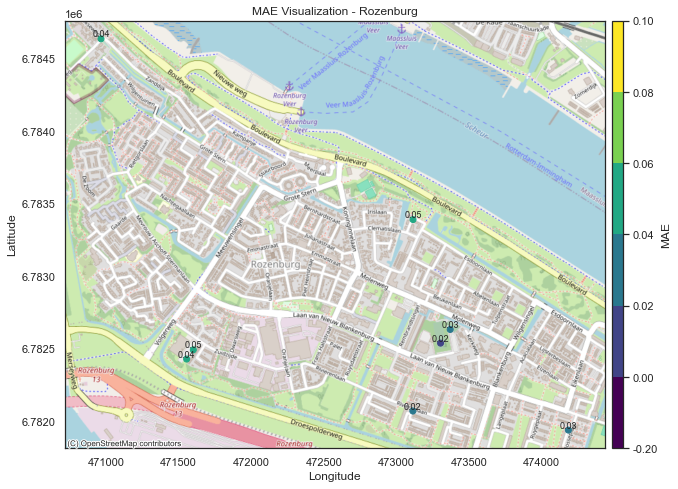
\includegraphics[width=1\linewidth]{frontmatter/Rozenburg-fig/newmae.png}
    \caption{Mean Absolute Error [meters] across Rozenburg, using a color-coded system to represent the calculated MAE for the eliminated monitoring wells. Based on EPSG:28992/Amersfoort RD New.}
    \label{maeroz}
\end{figure}

\clearpage

\subsubsection{Remaining Network}
After the network is reduced, 75\% of the monitoring wells will remain in the GWMN after reduction takes place. A geographical representation of the monitoring wells is available in figure \labelcref{afterroz}. The blue sites indicate the location of the existing monitoring wells. Initially, the GWMN of Rozenburg has a density of one monitoring well/11.17 hectares. After the reduction-optimization process, the network changes to one monitoring well/15.42 hectares.

\begin{figure}[htbp]
    \centering
    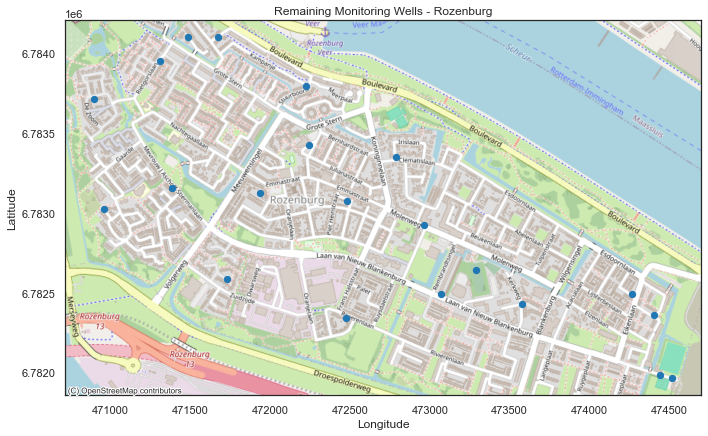
\includegraphics[width=1\linewidth]{frontmatter/Rozenburg-fig/newrem.png}
    \caption{Map depiction of the remaining monitoring wells in Rozenburg after following a 25\% reduction of the network. Based on EPSG:28992/Amersfoort RD New.}
    \label{afterroz}
    
\end{figure}

\clearpage

\section{Heijplaat}
\subsection{QGIS and PROWAT}
Figure \labelcref{summheij} represents a multi-colored scatter plot, showing the groundwater level [m NAP] over time [days]. Each colored dot represents an individual data point from a unique monitoring well, see legend on the right side of the figure. A wide array of groundwater levels is depicted, ranging from +1.0 to +3.5 m NAP. \\
\\
Plot \labelcref{summheij} visualizes the variation in groundwater levels between different monitoring wells. The legend explains a range of colors for the unique monitoring wells that counts to 14 in the study area Heijplaat. The function of the groundwater levels is indicated by the colored dot for every monitoring well. When no dot is present, it means no data is available for this specific measurement date. Several monitoring wells perform constant groundwater levels, while other monitoring wells have abundant fluctuations in their function. Dense clustering of data points might suggest that measurements were taken frequently over time. The variety of colors allows for the possibility to compare groundwater level fluctuations between monitoring locations within the neighborhood. \\
\\
\begin{figure}[htbp]
    \centering
    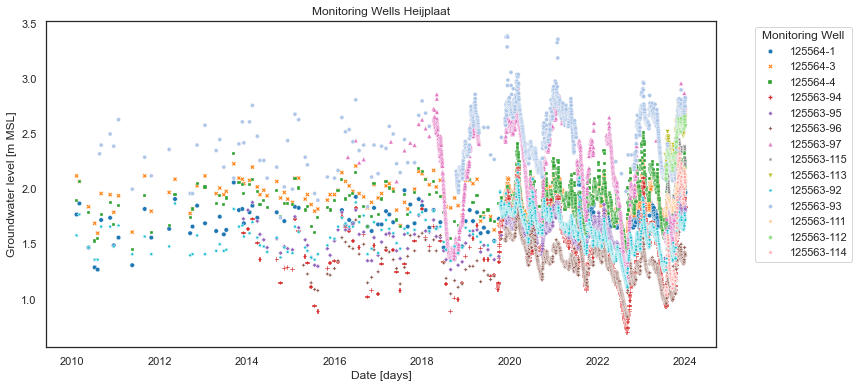
\includegraphics[width=0.75\linewidth]{frontmatter/Heijplaat-fig/heijoverzicht.png}
    \caption{Observed data for 14 monitoring wells in Heijplaat.}
    \label{summheij}
\end{figure}\\

\subsection{Pastas time series modeling}
Similarly to the plot in the section of Rozenburg, the bar plot displays the recharge rates [m/day] over a period from 2010-2024, figure \labelcref{R} . The y-axis quantifies the recharge rate with values ranging from 0 to 0.07 m/day. The bars show variability in recharge rates over time, where some years experience peaks in recharge (higher recharge rates), which can be due to increased precipitation. As can be seen from figure \labelcref{R}, the data is dense, indicating frequent measurements by KNMI. The pattern of the bars reflects seasonal changes. Lower values of recharge are more frequently observed than high outliers, possibly indicating a baseline level of recharge over the years. Two additional figures (\labelcref{P} and \labelcref{ET}) of the precipitation and potential evaporation data are visualized as well. The data of these figures is combined to determine the recharge rate in the municipal area. 
\begin{figure}[htbp]
    \centering
    \includegraphics[width=0.75\linewidth]{frontmatter/Heijplaat-fig/Recharge.png}
    \caption{Recharge [m/day] over a period of 2010-2024, measured by KNMI weather station 344 in Rotterdam, The Netherlands.}
    \label{R}
\end{figure} 
\begin{figure}[htbp]
    \centering
    % First figure
    \begin{minipage}{0.45\textwidth}
        \centering
        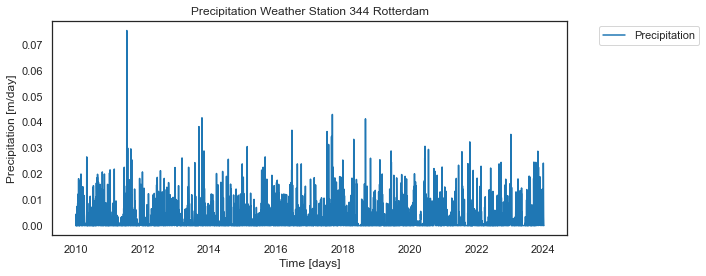
\includegraphics[width=\linewidth]{frontmatter/Heijplaat-fig/P.png}
        \caption{Precipitation [m/day] over a period of 2010-2024, measured by KNMI weather station 344 in Rotterdam, The Netherlands.}
        \label{P}
    \end{minipage}\hfill
    % Second figure
    \begin{minipage}{0.45\textwidth}
        \centering
        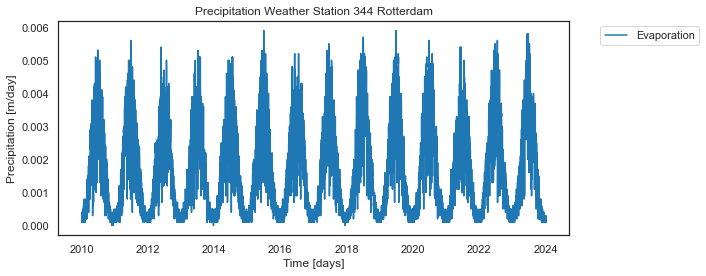
\includegraphics[width=\linewidth]{frontmatter/Heijplaat-fig/ET.png}
        \caption{Potential evaporation [m/day] over a period of 2010-2024, measured by KNMI weather station 344 in Rotterdam, The Netherlands.}
        \label{ET}
    \end{minipage}
\end{figure}
\newpage
\subsubsection{Reversed forecasting}
Reversed forecasting, or also known as backcasting, of the observed GWL data is a feature in the Pastas Python package. The process is applied for every unique monitoring well within the case study area. For every well, three types of visualizations are generated: 1) Backcasting for data logger data; 2) Backcasting for the manually collected data; 3) A combination figure of figures 1 and 2 combined, see figures \labelcref{dlheij}-\labelcref{combiheij}. Monitoring well 125563-97 shows an example of the three visualized figures. The following applies for all three figures: The x-axis includes a period of 2010-2024 and the y-axis shows the simulated GWL data [m NAP].

\begin{figure}[htbp]
    \centering
    % First figure
    \begin{minipage}{0.32\textwidth}
        \centering
        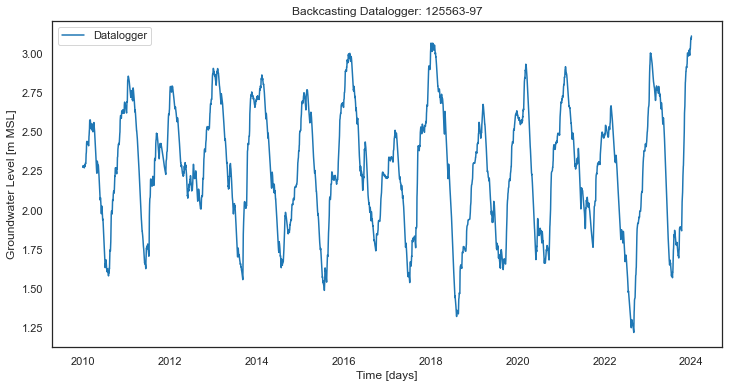
\includegraphics[width=\linewidth]{frontmatter/Heijplaat-fig/Figure 2024-03-12 094846 (48).png}
        \caption{Reversed forecasting data based on data logger data for monitoring well 125563-97.}
        \label{dlheij}
    \end{minipage}
    \hfill
    % Second figure
    \begin{minipage}{0.32\textwidth}
        \centering
        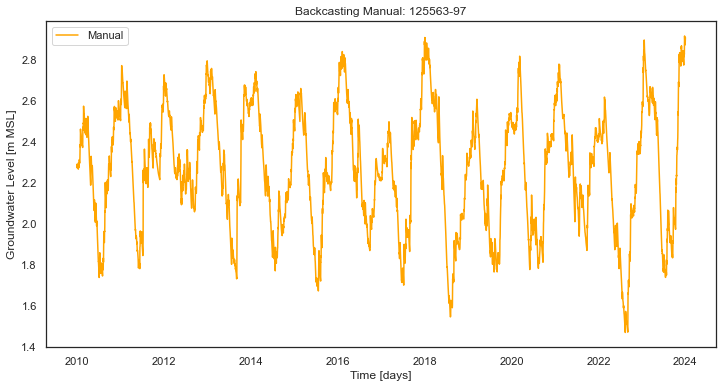
\includegraphics[width=\linewidth]{frontmatter/Heijplaat-fig/Figure 2024-03-12 094846 (62).png}
        \caption{Reversed forecasting data based on manual measurement data for monitoring well 125563-97.}
        \label{hpheij}
    \end{minipage}
    \hfill
    % Third figure 
    \begin{minipage}{0.32\textwidth}
        \centering
        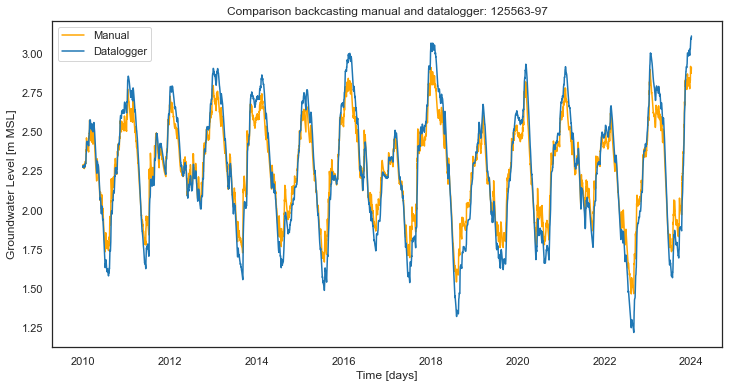
\includegraphics[width=\linewidth]{frontmatter/Heijplaat-fig/Figure 2024-03-12 094846 (76).png}
        \caption{Reversed forecasting data based on manual measurement data and datalogger data for monitoring well 125563-97.}
        \label{combiheij}
    \end{minipage}
\end{figure}

\newpage
\subsubsection{Performance metrics}
The bar plot \labelcref{bar1heij} and \labelcref{bar2heij} shows the two metrics RMSE and R$^2$ for all unique monitoring wells. In figure \labelcref{bar1heij}, a first overview is given of the t-Test with a distinction between RMSE and $R^2$ and an additional distinction between data loggers and manually collected wells. In figure \labelcref{bar1heij}, the $R^2$ value (orange bar) of all monitoring wells seem higher than the values of the RMSE (blue bar) of the same monitoring wells. Figure \labelcref{bar2heij} encompasses four categories: 1) manual-rmse; 2) manual-rsq; 3) datalogger-rmse; 4) datalogger-rsq. From this figure it is not clear if one of the datagroups has a better model performance, the performance of every model statistic differs between the monitoring wells. An additional bar plot, figure \labelcref{barevpheij}, describes the EVP [\%] across the dataset. The EVP compares the variance of the observed data and the variance of the residual data across the 14 monitoring wells \cite{asmuth-2021}. It is not clear how the values relate to each other, because there is a distinction between the datalogger and manual collection method. A low EVP might indicate that data could be missing in the dataset, the spatial pattern could be a reason. A statistical t-Test is a follow-up to identify and statistically substantiate the difference in performance between datagroups. Based on the results of the barplot, the decision was made to execute further statistical tests. A Welch's t-Test was carried out, leading to the following results. The Welch's t-Test uses an \(alpha=0.05\).

\begin{figure}[htbp]
    \centering
    % First figure
    \begin{minipage}{0.48\textwidth}
        \centering
        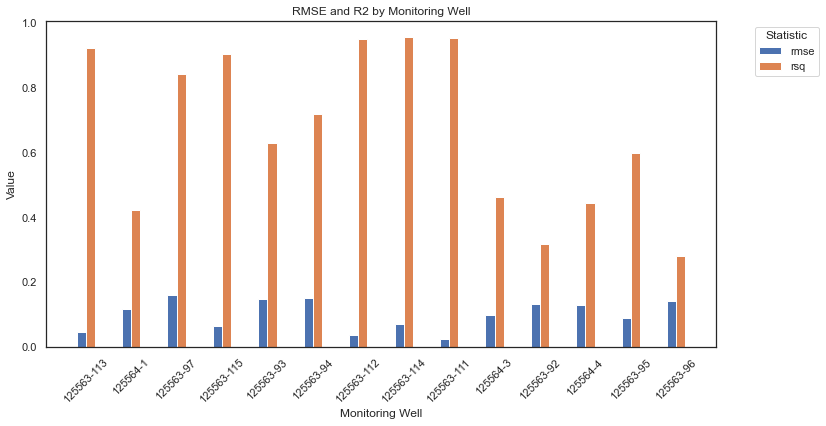
\includegraphics[width=\linewidth]{frontmatter/Heijplaat-fig/rmr2heij.png}
        \caption{Bar plot showing the metrics RMSE and $R^2$ for 14 monitoring wells.}
        \label{bar1heij}
    \end{minipage}\hfill
    % Second figure
    \begin{minipage}{0.48\textwidth}
        \centering
        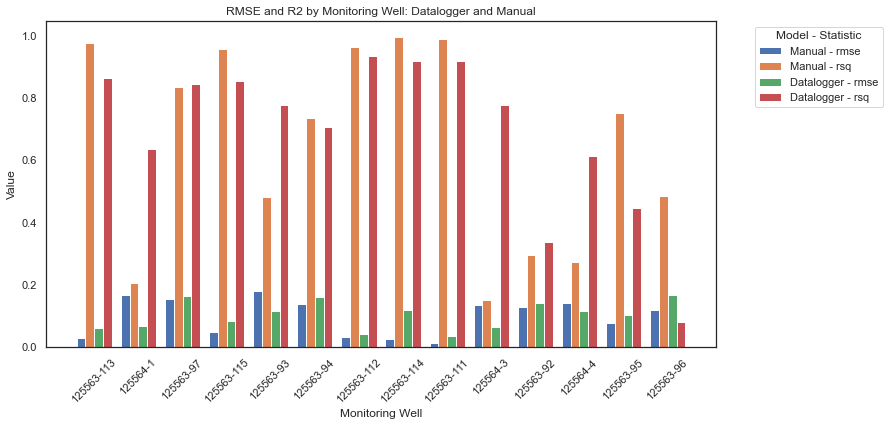
\includegraphics[width=\linewidth]{frontmatter/Heijplaat-fig/rmser2heij.png}
        \caption{Bar plot showing metrics RMSE and $R^2$ for 14 monitoring wells with a division in data logger and manual collection method.}
        \label{bar2heij}
    \end{minipage}\hfill
    % Third figure
    \begin{minipage}{0.48\textwidth}
        \centering
        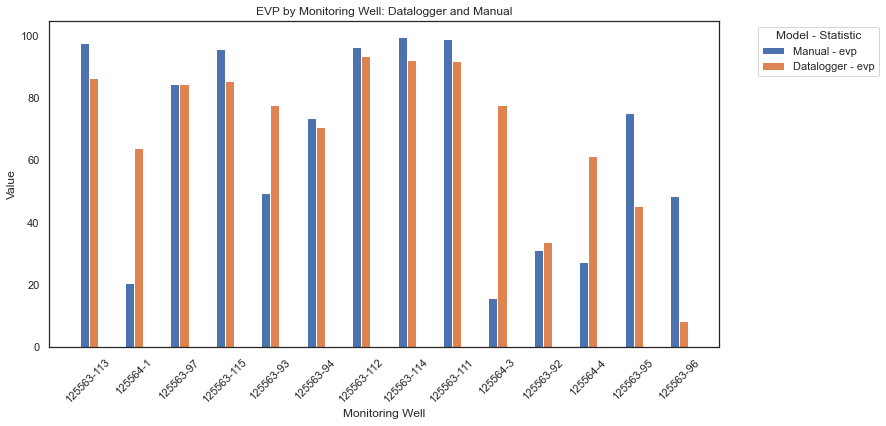
\includegraphics[width=\linewidth]{frontmatter/Heijplaat-fig/evpheij.png}
        \caption{Bar plot showing metric EVP for 14 monitoring wells.}   
        \label{barevpheij}
    \end{minipage}
\end{figure}
\noindent
Figure \labelcref{welchheij} displays the result of the Welch's t-Test, based on \(alpha = 0.05.\) The results of the performance metrics are labeled as RMSE, $R^2$, and EVP. Each performance metric provides the results of the t-statistic and p-value of the Welch's statistical test. The RMSE (blue section), explains that the t-statistic is positive. The p-value is higher than \(alpha = 0.05\). A p-value lower than the set alpha normally explains that a significant difference is present between the data loggers and manual collection method. The $R^2$ (orange section) explains that the t-statistic is negative, indicating a lower mean $R^2$ for the data loggers than the manual collection method. The p-value is slightly higher than \(alpha = 0.05\), indicating no significant difference. The last metric is the EVP (green section). The t-statistic of the EVP has a negative value, suggesting that the data loggers might have a lower mean EVP than the manual collection method. The p-value is higher than the set alpha, but results in no significant difference. 

\clearpage

\begin{figure}[htbp]
    \centering
    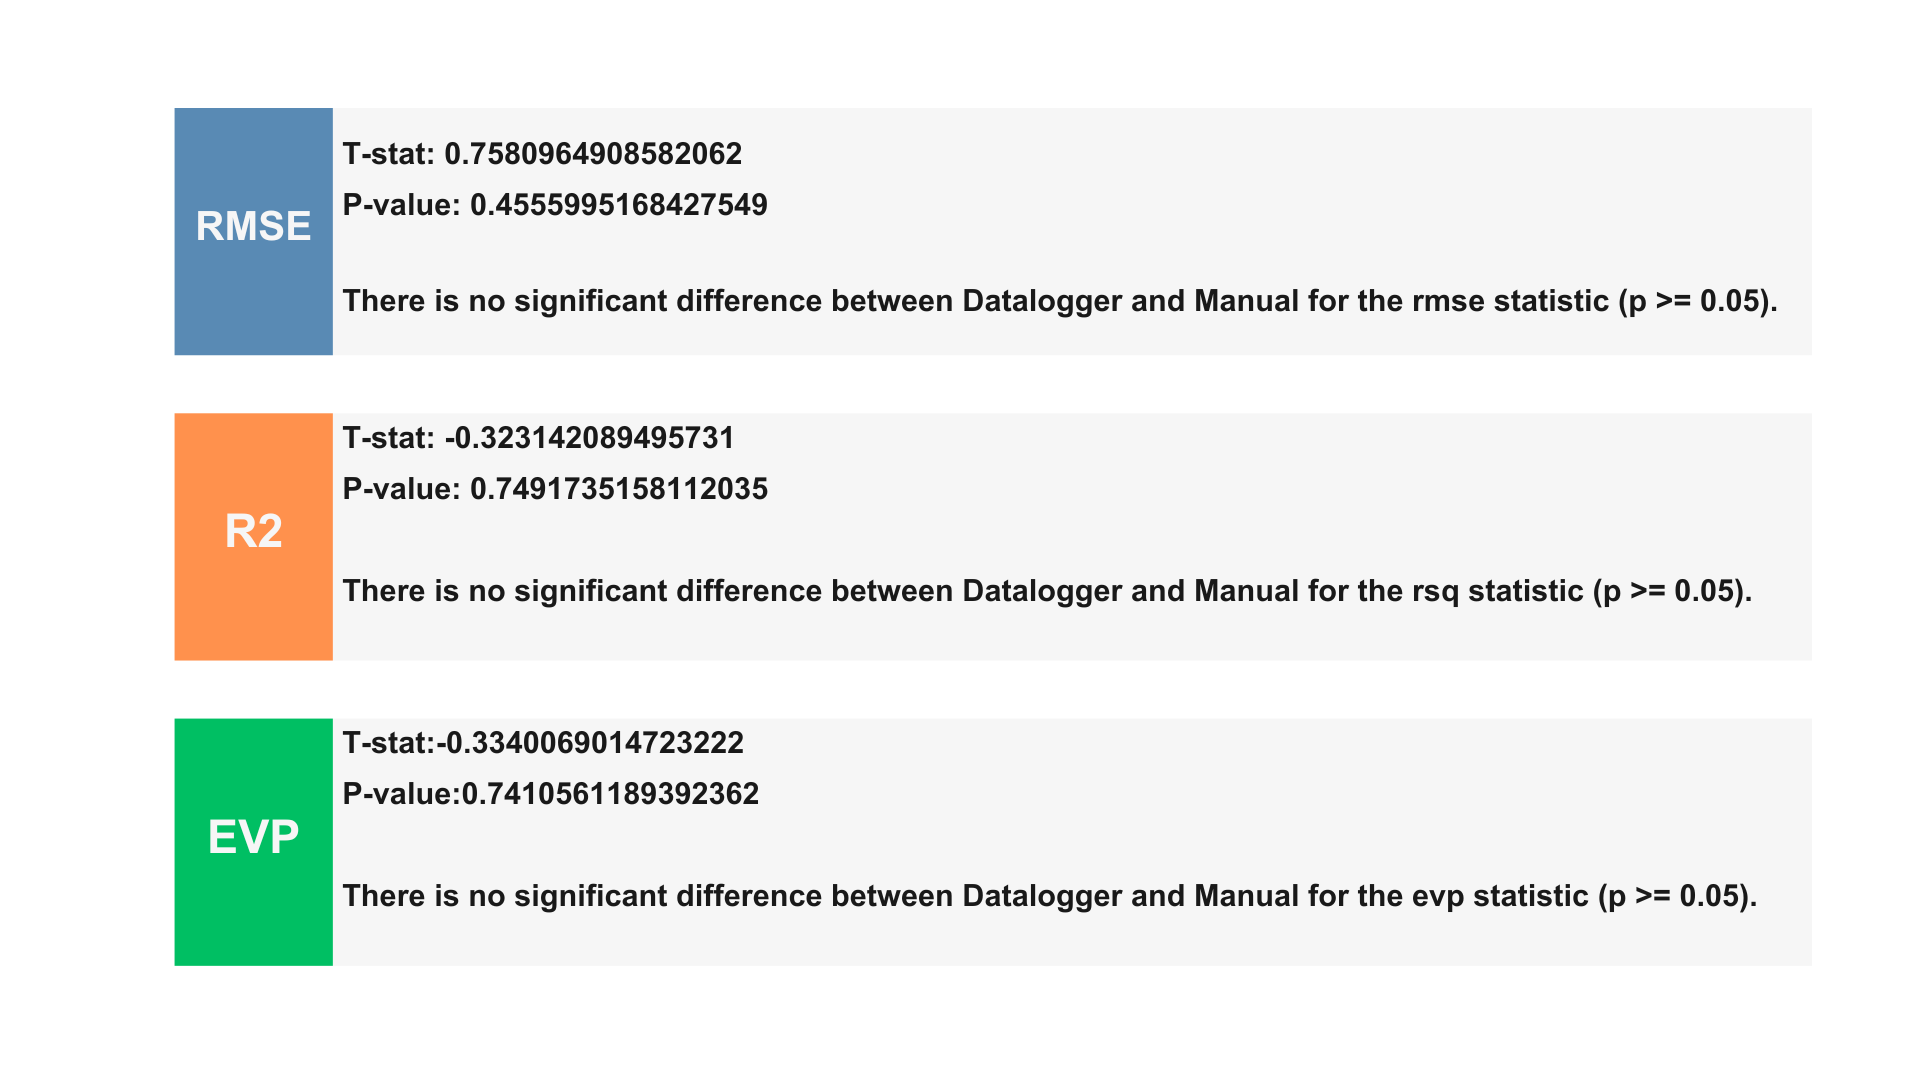
\includegraphics[width=0.80\linewidth]{frontmatter/Heijplaat-fig/statheij.png}
    \caption{Overview of the performance of RMSE, $R^2$, EVP after the Welch's t-test and the difference between data loggers and manual collection method.} 
    \label{welchheij}
\end{figure}
\noindent
The Welch's t-Test does not reveal substantial discrepancies between the data groups. None of the p-values are below the threshold value of 0.05. Despite statistical significance, factors as data availability and reliability are decisive. Hence, the data logger group is chosen, merging observed and simulated data into one dataset and excluding the manual measurement from the research.

\subsubsection{Creation of a new data frame}
The scatter plot \labelcref{scatterheij} below visualizes the observed data logger data with the blue scatter and the simulated data of the data logger is visualized by the orange scatter. On the x-axis the time period [days] is shown and on the y-axis the groundwater level [m NAP]. Figure \labelcref{scatterheij} visualizes only monitoring well 125563-97, the remaining monitoring wells of the neighborhood are available through \href{https://github.com/hannahwillemijn9/GWMNO-Rotterdam.git}{Github}.

\begin{figure}[htbp]
    \centering
    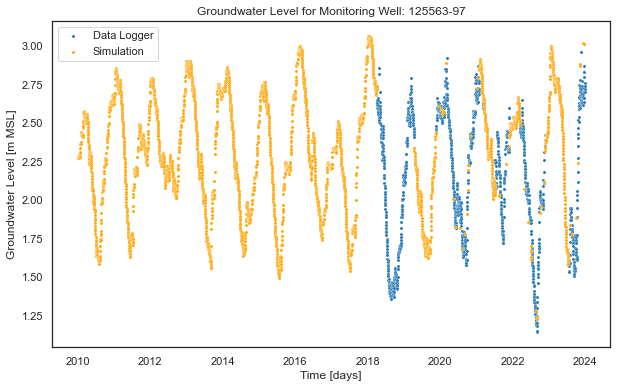
\includegraphics[width=0.80\linewidth]{frontmatter/Heijplaat-fig/Figure 2024-03-12 094846 (94).png}
    \caption{Scatter plot of simulated and observed data by data loggers for monitoring well 125563-97. The x-axis shows a period of 2010-2024 and the y-axis shows a range of +1.25 to 3.0 meters NAP.}  
    \label{scatterheij}
\end{figure}

\subsection{QR factorization}
Using QR factorization as foundation, a hierarchical list of the monitoring wells in Heijplaat can be created. The optimal reduction percentage is determined and reduction tests can be executed, resulting in an overview of eliminated monitoring wells and their capability to reconstruct future groundwater levels in the network.

\subsubsection{1D hydrograph data}
Figure \labelcref{gwlheij} is a geographical representation visualizing the spatial distribution of monitoring wells in the neighborhood Heijplaat. Within the map, a scatter plot with a color scale represents the groundwater level measurements taken at the monitoring wells. The groundwater level has a range between -0.5 m to +3.0 m NAP. Each monitoring well represents a location as well as the color of monitoring well represents the value on the color scale. At the south side of the neighborhood, the GWL is increasing from approximately 2.0 meters to 3.0 meters [NAP]. For Heijplaat the increasing GWL can not necessarily be defined through the elevation difference of the ground level, a digital terrain model of Heijplaat is displayed in figure \labelcref{ahnheij}. 

\begin{figure}[htbp]
    \centering
    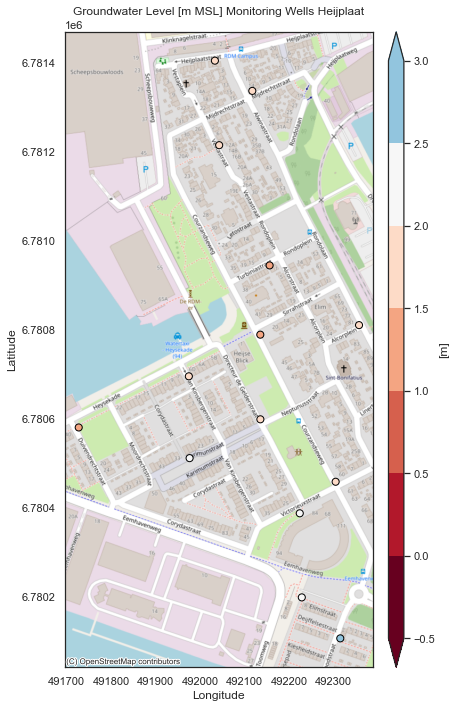
\includegraphics[width=0.50\linewidth]{frontmatter/Heijplaat-fig/gwlheij.png}
    \caption{Groundwater level [m NAP] across Heijplaat, using a color-coded system to represent the mean GWL observations for 14 monitoring wells. Based on EPSG:28992/Amersfoort RD New.}
    \label{gwlheij}
\end{figure}


\clearpage

\subsubsection{Sampling data}
Preprocessing of the data includes transforming the data frame into an array, implementing both global and local centering methods, and splitting the dataset into an 80/20 ratio training and test set distribution. The result of the preprocessing is as follows, see table \labelcref{dataheij}.

\begin{table}[htbp]
\centering
\caption{Summary of sampling data.}
\label{dataheij}
\begin{tabular}{|l|l|}
\hline
\textbf{Parameter}                           & \textbf{Value}                                \\ \hline
Sampling period                              & 2020-01-02 00:00:00 to 2024-01-01 00:00:00   \\ \hline
Number of samples                            & 1462                                          \\ \hline
Number of features (sensors)                 & 14                                            \\ \hline
Shape of X (samples, sensors)                & (1462, 14)                                    \\ \hline
Min. and max. value                          & 0.7 [m]; 3.36 [m] \\ \hline
Train data, Test data                        & 1169 , 293                                   \\ \hline
Train data, Test data (percentage)           & 80\%, 20\%                                  \\ \hline
\end{tabular}
\end{table} 

\subsubsection{Hierarchy of monitoring wells}
A geographical representation of data points plotted on a x,y coordinate system is visualized in figure \labelcref{rankheij}. The horizontal axis is labeled as longitude and the vertical axis is labeled as latitude. The data points are scattered across the study area within the neighborhood Heijplaat. Each monitoring well is color-coded according to the color bar on the right side of the plot. The color indicates the rank of each monitoring well and has a range between dark blue for the lowest values (1) to yellow for the highest values (14). The distribution of the color code does not follow a clear pattern within the neighborhood. Some clusters of higher or lower ranked monitoring wells are present. The monitoring wells with additional value are marked blue, while the monitoring wells that likely do not have additional value to the network are marked yellow. The most redundant monitoring wells appear to be located towards the southern edge of the neighborhood. At the southern side, monitoring wells are clustered and address a region of low data variability and flashiness. 

\begin{figure}[htbp]
    \centering
    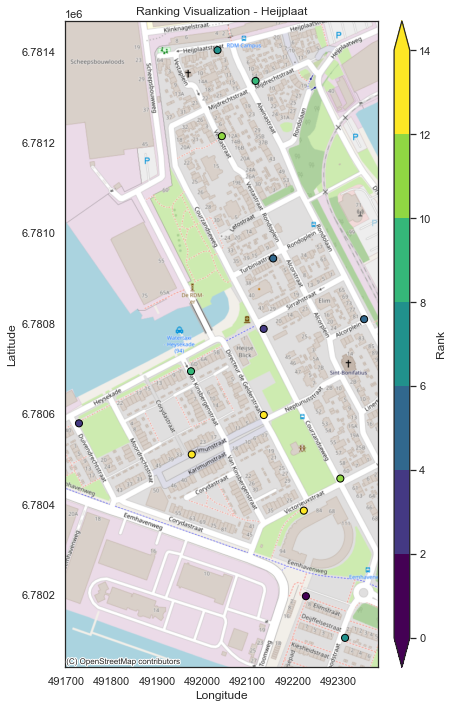
\includegraphics[width=0.75\linewidth]{frontmatter/Heijplaat-fig/rankheij.png}
    \caption{Visualization of the hierarchical list of 14 monitoring wells across Heijplaat. Based on EPSG:28992/Amersfoort RD New.}
    \label{rankheij}
\end{figure}

\clearpage

\subsubsection{Determining the optimal reduction rate}
Figures \labelcref{heij10}-\labelcref{heij90} visualize the Reconstruction Error of Heijplaat, plotting the number of monitoring wells on the x-axis against the root mean square error (RMSE) in meters on the y-axis. The line graph shows a decreasing function as the number of monitoring wells increases and the RMSE decreases, suggesting that more monitoring wells contribute to a lower reconstruction error in the data. In the figures, the orange marked point marks the optimal number of monitoring wells where the reconstruction error reaches the threshold that is indicated by the orange line. The threshold is an acceptable level of RMSE for the reconstruction process. The original groundwater monitoring network of Heijplaat includes 14 monitoring wells. 
\newline
Starting with a reduction percentage of 10\%, the network is reduced to 12 monitoring wells with a reconstruction error of below 0.02 meters, see figure \labelcref{heij10}. Figure \labelcref{heij25} describes a reduction of 25\% and explains that a number of 10 monitoring wells is the most optimal with a removal of 4 monitoring wells. The RMSE is calculated to determine the optimal number of monitoring wells in the neighborhood. Figure \labelcref{heij50}, demonstrates a function based on a reduction percentage of 50\%. The RMSE decreases as more monitoring wells are added to the network. At the point of n=7 on the x-axis, an orange dot is indicated. Beyond this point, the decrease in RMSE slows down, suggesting returns on error reduction after a specific number of monitoring wells is reached. 
\begin{figure}[htbp]
    \centering
    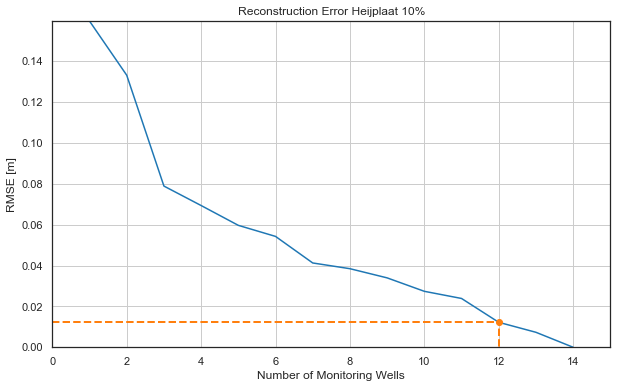
\includegraphics[width=0.5\linewidth]{frontmatter/Heijplaat-fig/new10.png}
    \caption{RMSE based on a network reduction of 10\%. The optimal number of wells is 12.}
    \label{heij10}
\end{figure}

\begin{figure}[htbp]
    \centering
    \begin{minipage}{0.45\linewidth}
        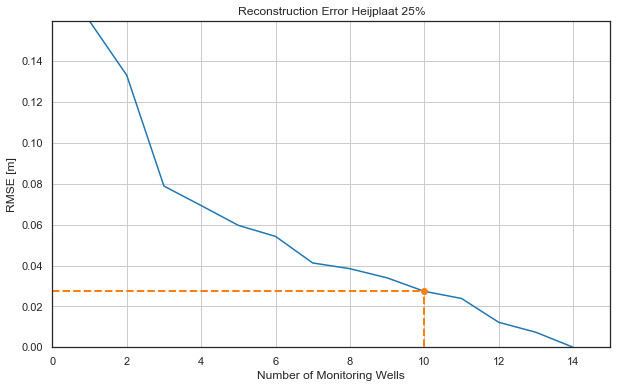
\includegraphics[width=\linewidth]{frontmatter/Heijplaat-fig/new25.png}
        \caption{RMSE based on a network reduction of 25\%. The optimal number of wells is 10.}
        \label{heij25}
    \end{minipage}
    \hfill
    \begin{minipage}{0.45\linewidth}
        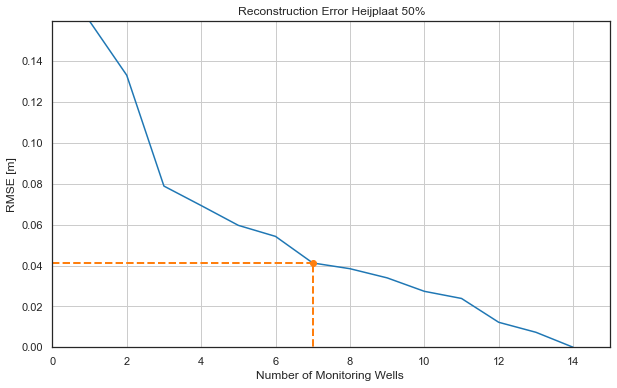
\includegraphics[width=\linewidth]{frontmatter/Heijplaat-fig/new50.png}
        \caption{RMSE based on a network reduction of 50\%. The optimal number of wells is 7.}
        \label{heij50}
    \end{minipage}
\end{figure}
\noindent
Figure \labelcref{heij75}, displays a similar function where the RMSE decreases as the number of monitoring wells increases. The RMSE declines as the monitoring well count reaches the point above 3 monitoring wells. This is the point marked with the orange dashed line. The line marks the optimal number of monitoring wells where the reconstruction error reaches the threshold value. The threshold value is an acceptable level of RMSE for the reconstruction process. Initially, Heijplaat includes 14 monitoring wells. The results of the RMSE explains that only 3 monitoring wells remain in the network, 11 monitoring wells have to be removed from the local network if a reduction of 75\% is being used in the approach. A reduction percentage of 75\% explains an equilibrium state between the number of monitoring wells and the reconstruction error that is achieved. 
\newline
Continuing with figure \labelcref{heij90}, the reconstruction error for a reduction of 90\% is displayed. The figure plots the number of monitoring wells on the x-axis against the RMSE in meters on the y-axis. The line graph shows a decreasing function in the RMSE as the number of monitoring wells increases. The orange marked point, marks the optimal number of monitoring wells where the reconstruction error reaches the threshold value that is indicated by the orange line. The threshold value is an acceptable level of RMSE for the reconstruction process. Initially, Heijplaat includes 14 monitoring wells. The results of the RMSE calculation explains that a number of  1 monitoring well will remain in the network, while 13 monitoring wells will be eliminated from the network.

\begin{figure}[htbp]
    \centering
    \begin{minipage}{0.45\linewidth}
        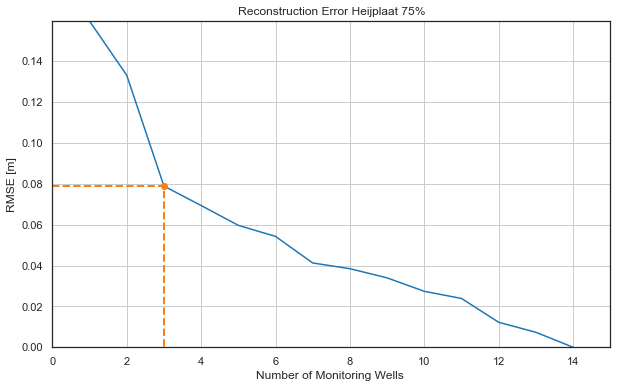
\includegraphics[width=\linewidth]{frontmatter/Heijplaat-fig/new75.png}
        \caption{RMSE based on a network reduction of 75\%. The optimal number of wells is 3.}
        \label{heij75}
    \end{minipage}
    \hfill
    \begin{minipage}{0.45\linewidth}
        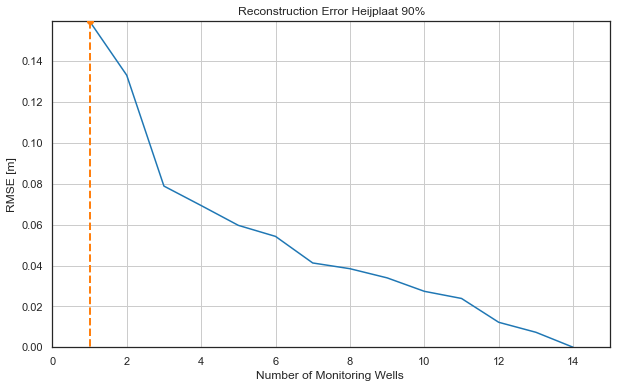
\includegraphics[width=\linewidth]{frontmatter/Heijplaat-fig/new90.png}
        \caption{RMSE based on a network reduction of 90\%. The optimal number of wells is 1.}
        \label{heij90}
    \end{minipage}
\end{figure}

\subsubsection{The optimal reduction rate}
The optimal reduction rate for a monitoring network consisting of 14 monitoring wells counts up to a value where the RMSE reaches a point of stabilization. Figure \labelcref{rmseheij} visualizes all reduction percentages between a range of 10-90\% with their corresponding reconstruction error. 
%The upper values of each reduction rate correlate to the MAE, while the lower values, with the connecting dashed-line, describes the reconstruction error.  
A reduction percentage of 25\% implies that the optimal number of monitoring wells is 10, meaning that 4 monitoring wells might be eliminated from the network, see figure 5.48. Additionally, the RMSE counts up to 0.027 meters. As stated in the chapter \labelcref{chapter:RM} the reconstruction capability of the eliminated monitoring wells is tested through the creation of hydrographs. In figures \labelcref{hwell1}-\labelcref{hwell4}, hydrographs are shown. The hydrographs include a measured (blue line) and reconstructed (orange line) function. The reconstructed functions are based on observed data and the Goodness-of-Fit of the model. Performance metrics regarding the MAE, RMSE, $R^2$ and rBIAS determine the Goodness-of-Fit of the functions, they are available underneath the figures \labelcref{hwell1}-\labelcref{hwell4}. 

\begin{figure}[h]
    \centering
    \includegraphics[width=0.60\linewidth]{frontmatter/Heijplaat-fig/redscenheij.png}
    \caption{Overview of RMSE for a range of reduction (10-25-50-75-90\%).}
    \label{rmseheij}
\end{figure}
\newpage
\noindent
As can be seen from the figures, the plots have comparable functions; a decreasing groundwater level from April to July 2023. An increase occurs in July towards mid August 2023. During the start of Fall, a small increase in groundwater level occurs in October with strong increases in November and December 2023. In January 2024, the groundwater level is just as high as at the beginning of November 2023. Based on the performance metrics of the potentially eliminated monitoring wells, it can be seen that the MAE and RMSE are constant values throughout the network. The MAE reaches a value of 0.04 meters and the RMSE counts up to 0.05 meters as well. The coefficient of determination differs for every monitoring well, but ranges between 0.87 and 0.96. An average $R^2$ of 0.925 [] is calculated.
\begin{figure}[h]
    \centering
    % Eerste rij
    \begin{minipage}{0.48\linewidth}
        \includegraphics[width=\linewidth]{frontmatter/Heijplaat-fig/125563111heij.png}
        \caption{Eliminated monitoring well: 125563-111.}
        \label{hwell1}
    \end{minipage}
    \hfill
    \begin{minipage}{0.48\linewidth}
        \includegraphics[width=\linewidth]{frontmatter/Heijplaat-fig/1255641heij.png}
        \caption{Eliminated monitoring well: 125564-1.}
        \label{125564-1}
    \end{minipage}
    
    % Tweede rij
    \begin{minipage}{0.48\linewidth}
        \includegraphics[width=\linewidth]{frontmatter/Heijplaat-fig/125563113heij.png}
        \caption{Eliminated monitoring well: 125563-113.}
        \label{125563-113}
    \end{minipage}
    \hfill
    \begin{minipage}{0.48\linewidth}
        \includegraphics[width=\linewidth]{frontmatter/Heijplaat-fig/1255643heij.png}
        \caption{Eliminated monitoring well: 125564-3.}
        \label{hwell4}
    \end{minipage}
\end{figure}
\newline
The measured and reconstructed groundwater levels are tested with the Welch's t-Test to determine whether there is a case of a significant difference between the measured and reconstructed groundwater levels. The results are displayed in table \labelcref{theij}.  For Heijplaat, 3 out of 4 eliminated monitoring wells experience a significant difference between the measured and reconstructed groundwater level data. This means that the p-values of the monitoring wells are lower than \(alpha = 0.05\).
\begin{table}[htbp]
    \centering
        \caption{Overview of statistical results of the eliminated monitoring wells with a network reduction of 25\%. The overview explains the p-value of the monitoring wells if they experience a significant difference between the observed and reconstructed data. }
    \begin{tabular}{|c|c|} \hline  
         Monitoring Well& Result t-Test\\ \hline  
         125563-111& No significant difference 
(p-value = 0.134)\\ \hline  
         125563-113& Significant difference (p-value = 0.000)\\ \hline  
 125564-1&Significant difference (p-value = 0.000)\\ \hline 
         125564-3& Significant difference (p-value = 0.000)\\ \hline 
    \end{tabular}
    \label{theij}
\end{table}
\newpage
\noindent
Continuing with a box plot of the coefficient of determination, the $R^2$. Box plot \labelcref{boxheij} visualizes the distribution of the $R^2$ across the dataset after a reduction of 25\% took place. On the y-axis, the score in meters is shown, which ranges between 0.873 and 0.963. The orange line explains a median value of 0.938 []. The whiskers at the bottom and top of the box do not have equal lengths. The bottom whisker ranges from 0.873 to 0.917, while the whisker at the top ranges from 0.949 to 0.963 [].

\begin{figure}[htbp]
    \centering
    \includegraphics[width=0.50\linewidth]{frontmatter/Heijplaat-fig/boxheji.png}
    \caption{Performance metric $R^2$. The orange line indicates the median value. The y-axis ranges from 0.928 to 0.987 [].}
    \label{boxheij}
\end{figure}

\subsubsection{Mean Absolute Error of Reduction}
Based on a reduction percentage of 25\%, reconstruction hydrographs could be plotted in figures \labelcref{hwell1}-\labelcref{hwell4}. The extent to which the reconstructed groundwater level data corresponds to the actual observed data can be determined by the mean absolute error [meters]. The mean absolute error is calculated for every eliminated monitoring well. A color rank visualizes the level of the calculated mean absolute error in figure \labelcref{maeheij}. Blue indicates a low MAE, while yellow indicates a high MAE. The visualization enables the identification of monitoring wells with higher or lower predictive accuracy, which could influence decision-making regarding the placement of future monitoring wells or the scope of maintenance efforts on existing wells. The MAE measures indirectly the performance of the monitoring well regarding data reconstruction. A high MAE in a network of lower MAE values can suggest a vulnerable monitoring well for external environmental factors. Monitoring wells with a high MAE can not be reproduced easily, because the prediction can be unreliable. The monitoring well that is marked with a green color indicates a higher MAE value compared to the other monitoring wells. 

\begin{figure}[htbp]
    \centering
    \includegraphics[width=0.75\linewidth]{frontmatter/Heijplaat-fig/maeheij.png}
    \caption{Mean Absolute Error [meters] across Heijplaat, using a color-coded system to represent the calculated MAE for the eliminated monitoring wells. Based on EPSG:28992/Amersfoort RD New.}
    \label{maeheij}
\end{figure}
\clearpage

\subsubsection{Remaining Network}
After the network is reduced, 75\% of the monitoring wells will remain in the GWMN after reduction takes place. A geographical representation of the monitoring wells is available in figure \labelcref{afterheij}. The blue sites indicate the location of the remaining monitoring wells in the network. Originally, the neighborhood Heijplaat had a density of one monitoring well/2.78 hectares. After the reduction-optimization process, the network changes to one monitoring well/3.90 hectares. 
\begin{figure}[htbp]
    \centering
    \includegraphics[width=0.75\linewidth]{frontmatter/Heijplaat-fig/remheij.png}
    \caption{Map depiction of the remaining monitoring wells in Heijplaat after following a 25\% reduction of the network. Based on EPSG:28992/Amersfoort RD New.}
    \label{afterheij}
\end{figure}



